\documentclass{lab_sheet}
\usepackage{booktabs,caption}
\usepackage{multirow}
\usepackage[flushleft]{threeparttable}
\usepackage{tikz}
 \usetikzlibrary{shapes.geometric, arrows,positioning}
   \tikzstyle{process} = [rectangle, text width=3cm, minimum height=1cm,    text centered, draw=black, fill=orange!20]
   \tikzstyle{case} = [rectangle, text width=3cm, minimum height=1cm,    text centered, draw=black, fill=blue!20]
   \tikzstyle{decision} = [diamond, text width=3cm, minimum height=1cm, text centered, draw=black, fill=green!20]
   \tikzstyle{arrow} = [thick,->,>=stealth]


   \newcommand{\packetforward}{
   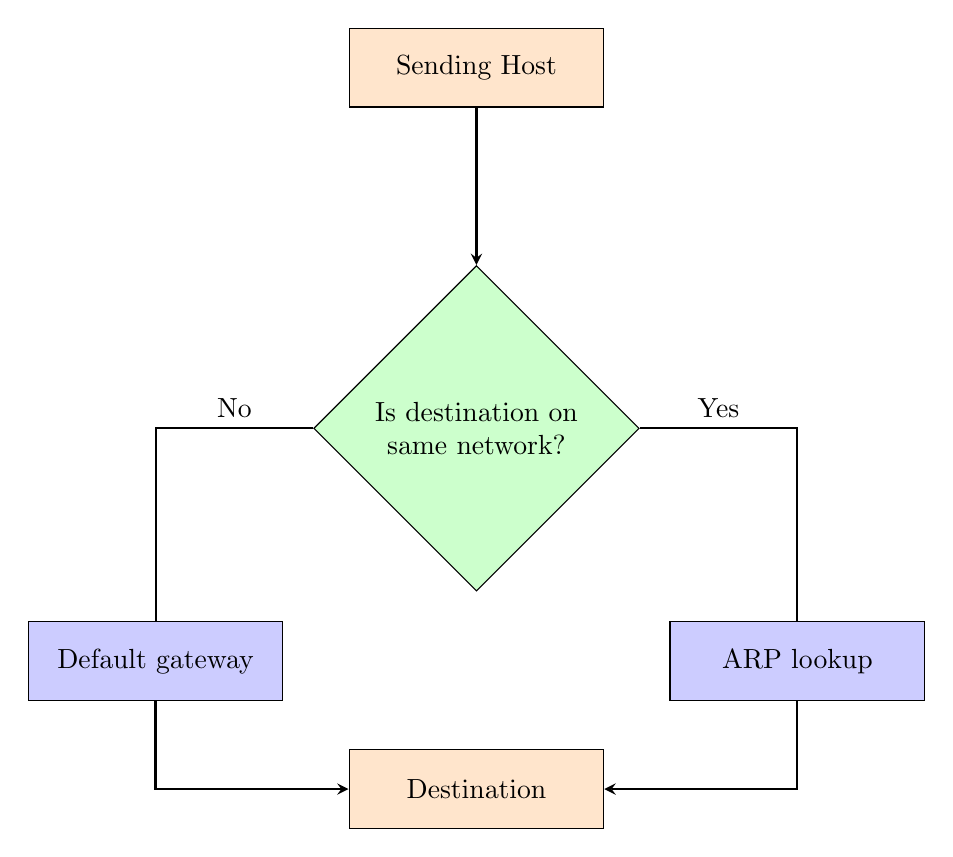
\begin{tikzpicture}[node distance=2cm]
   \node (host) [process] {Sending Host};
   \node (dec1) [decision, below=of host] {Is destination on same network?};
   \node (arp) [case, below right =of dec1] {ARP lookup};
   \node (gateway) [case, below left =of dec1] {Default gateway};
   \node (destination) [process, below =of dec1] {Destination};
   \draw [arrow] (host) -- (dec1);
   \draw [arrow,-] (dec1.west) -- ++(-2,0) node[midway,above]{No} |- (gateway.north);
   \draw [arrow,-] (dec1.east) -- ++(2 ,0) node[midway,above]{Yes} |- (arp.north);
   \draw [arrow] (gateway.south) -- ++ (0,-1) |- (destination.west);
   \draw [arrow] (arp.south) -- ++ (0,-1) |- (destination.east);
  \end{tikzpicture}
   }
\newcommand{\parameter}[1]{
    \begin{tabular}{C{3cm}C{2cm}C{2cm}C{2cm}C{2cm}}
        \toprule
        Router & hostname & console password & enable password& vty password\\
        \midrule
          #1 
          \bottomrule
       \end{tabular}
}
\newcommand{\setting}[2]{
    \begin{tabular}{C{3cm}C{5cm}C{5cm}}
        \toprule
          #1 & IP address & Subnet mask\\
          \midrule
          #2
          \bottomrule
       \end{tabular}
}

\newcommand{\ping}[1]{
    \begin{tabular}{||C{3cm}||C{5cm}||C{5cm}||}
        \toprule
          Sending Host & Destination & Ping status\\
          \hline
          #1
          \bottomrule
       \end{tabular}
}
\begin{document}
    \titlePage{Subnet Mask, Default Gateway and Static Routing}{November 12, 2020}
    \pagenumbering{gobble}
    \tableofcontents
    \pagebreak
    \listoffigures
    \pagebreak
    \listoftables
    \pagebreak
    \lstlistoflistings
    \pagebreak
    \pagenumbering{arabic}
    \section{Objectives}
    \begin{itemize}
        \item Familiarization with network and subnet mask.
        \item Familiarization with default gateway and its configuration.
        \item Familiarization with Routing: Static Routing and its configuration.
    \end{itemize}
    \section{Required Tools}
    \subsection{Cisco Packet Tracer}
    Cisco Packet Tracer is a visual simulation software developed and distributed by Cisco Systems. Packet Tracer is a cross platform tool that allows simulated environment for modern computer network and network topologies. 
    \section{Simulation Activities}
    The networks shown in Figure~\ref{fig:activitya}, \ref{fig:activityb} and \ref{fig:activityc} were created using packet tracer for the activities in the lab experiment. For sanity, the ping tests to and from group A (PC0, PC1 and PC2), group B (PC3, PC4 and PC5), and group C (PC6, PC7 and PC8) are represented by ping tests to and from PC0, PC3 and PC6 respectively. The observations for all the tests were conducted but only the selected ones are included in the report. The PCs are selected such that the observations represent the overall requirement of the activities.
    \begin{figure}[H]
        \centering
        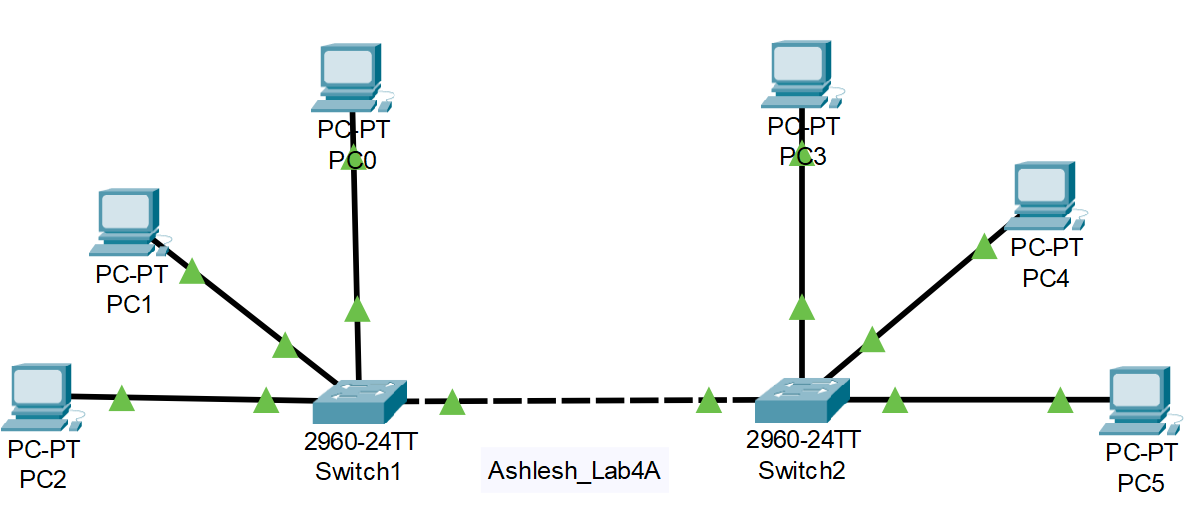
\includegraphics[scale=0.6]{./Figures/activitya.png}
        \caption{Simulated network for Activity A}
        \label{fig:activitya}
    \end{figure}
    \begin{figure}[H]
        \centering
        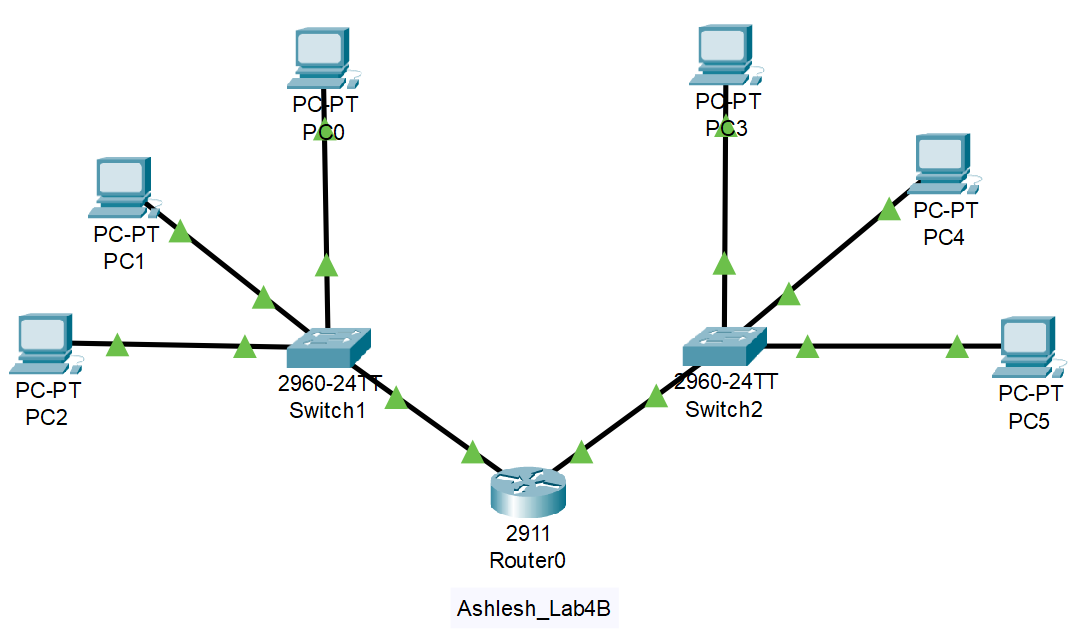
\includegraphics[scale=0.7]{./Figures/activityb.png}
        \caption{Simulated network for Activity B}
        \label{fig:activityb}
    \end{figure}
    \begin{figure}[H]
        \centering
        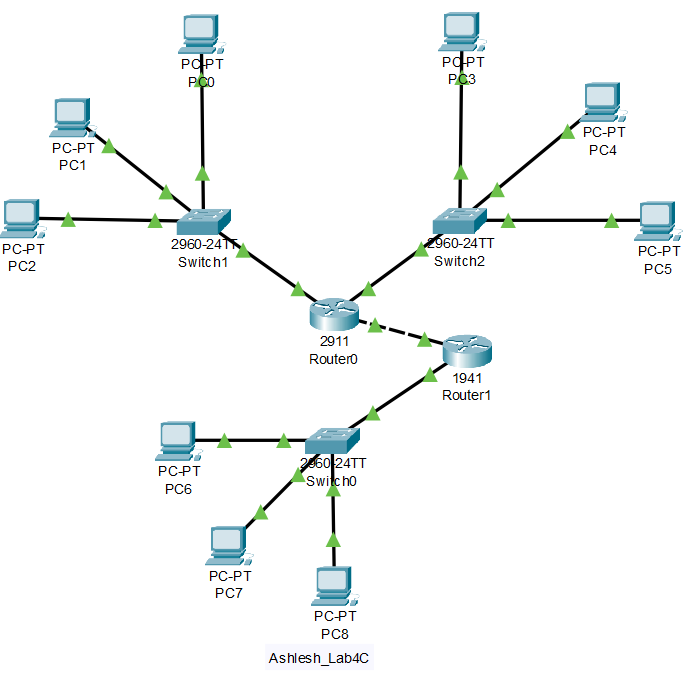
\includegraphics[scale=0.7]{./Figures/activityc.png}
        \caption{Simulated network for Activity C}
        \label{fig:activityc}
    \end{figure}
    \section{Exercises}
    \problem{What is a subnet mask? Why is it used? Explain with examples.}
    A subnet mask is a four-octet or 32-bit number that is used in networks to identify the network and host IDs of a 32-bit IP address. The subnet mask is used to mask certain bits in the IP address using bitwise ANDing to determine the network and host IDs.
    \begin{table}[H]
      \centering
      \begin{tabular}{C{2cm}C{3cm}C{6cm}C{3cm}}
        \toprule
          IP address Class & Decimal notation & Binary notation & Classless Inter-Domain Routing (CIDR) notation \\
          \midrule
          A & 255.0.0.0 & 11111111.00000000.00000000.00000000 & /8 \\
          B & 255.255.0.0 & 11111111.11111111.00000000.00000000 & /16\\
          C & 255.255.255.0 & 11111111.11111111.11111111.00000000 & /24\\
          \bottomrule
       \end{tabular}
\caption{Default subnet masks for IP classes}
\label{tbl:subnetmasks}
  \end{table}
    \begin{table}[H]
      \centering
      \begin{tabular}{C{2cm}C{4cm}C{4cm}C{4cm}}
        \toprule
         IP address Class & IP address & Network identifier & Host identifier\\
          \midrule
          A & a.b.c.d & a.0.0.0 & 0.b.c.d\\
          B & a.b.c.d & a.b.0.0 & 0.0.c.d \\
          C & a.b.c.d & a.b.c.0 & 0.0.0.d\\
          \bottomrule
       \end{tabular}
\caption{IP address class identifiers}
\label{tbl:classidentifier}
  \end{table}
  While the default subnet masks shown in Table~\ref{tbl:subnetmasks} are used in identifying the network and host IDs as in Table~\ref{tbl:classidentifier}, the usage of subnet mask isn't limited to that. Subnet masks are used to segment larger networks into subnetworking by a process called subnetting. The default mask allows for over 16 million hosts per network for class A, over 16 thousand for class B and 254 for class C. But these numbers are useless since physical networks aren't located on a single network segment. The use of custom subnet masks allow the network to be split up into multiple unique routable networks. For instance, by changing the subnet mask from 255.255.0.0 to 255.255.255.0, we have 254 unique networks that each support 254 hosts. 
  \begin{table}[H]
    \centering
    \begin{tabular}{C{2cm}C{6cm}C{6cm}}
      \toprule
      \multirow{2}{*}{IP address} & 200.200.20.2 & 200.200.20.34 \\
       \cline{2-3}
       & 11001000.11001000.00010100.00000010& 11001000.11001000.00010100.00100010\\
       \midrule
       Default Subnet mask &  \multicolumn{2}{c}{11111111.11111111.11111111.00000000} \\
        \midrule
        \multirow{2}{*}{Network ID}  & 11001000.11001000.00010100.00000000& 11001000.11001000.00010100.00000000\\
        \cline{2-3}
        & 200.200.20.0 & 200.200.20.0 \\
        \midrule
        Custom Subnet mask &  \multicolumn{2}{c}{11111111.11111111.11111111.11100000} \\
        \midrule
        \multirow{2}{*}{Network ID}  & 11001000.11001000.00010100.00000000& 11001000.11001000.00010100.00100000\\
        \cline{2-3}
        & 200.200.20.0 & 200.200.20.32 \\
        \bottomrule
     \end{tabular}
\caption{Subnetting using custom subnet mask}
\label{tbl:subnetting}
\end{table}
Another example of a subnet mask's usage illustrated in Table~\ref{tbl:subnetting}can be figured out by taking two addresses, 200.200.20.2 and 200.200.20.34. For a subnet mask of 255.255.255.0, both of these IPs are on the same network, 200.200.20.0. But if we change the subnet mask to 255.255.255.224, the IP 200.200.20.2 is on the network 200.200.20.0 and IP 200.200.20.34 is on the network 200.200.20.32.
    \problem{How does a sending host know whether the destination computer is on the same network or on the
    different network? How data packet is forwarded in each case from the sending host? Explain.}
    A sending host looking to communicate with a destination uses the subnet mask to determine whether the destination is in the same subnet as itself or in a different one. The bitwise ANDing of the IP address of the host and the subnet mask gives the network ID for the host. Similarly, the bitwise AND operation between the destination IP address and subnet mask identifies the network the destination is in. This is all performed by the sending host, based on which two of the following cases are possible,
    \subsubsection*{Host and destination in same subnet}
    If the destination is in the same subnet, i.e. is local to the host, the host uses the arp table to lookup the MAC address of the destination and directly communicates with the destination. 
    \subsubsection*{Host and destination in different subnet}
    If the destination is in a different subnet, i.e. is rempte to the host, the host forwards the packet to the default gateway which then uses the route tables to communicate with the destination.
    \begin{figure}[H]
      \centering
      \packetforward
      \caption{Data packet forwarding from host to destination}
      \label{fig:datapckt}
    \end{figure}
    \problem{What is a routing? Explain static routing and configuration of static routing in a router with its
    syntax and functions. Also mention how the routing table of a router can be observed.}
    Routing is a process of determining the best way for a packet to move from one network to another. It is a process used by a router to route packets based on the packet header and routing table.\\
    A router makes routing decisions based on which the packets are forwarded to the remote network. Static routing is one such method for routing. It is a technique where the network administrator adds non-adaptive routes manually into the routing table. The routes aren't to be modified or changed by the router based on network status. The use of static routing technique is useful for networks that require control over the routes that a packet takes, which ensures security during communication. The routes are manually added on the routing table using the syntax enlisted in Listing~\ref{lst:syntaxrouting}.
    \lstinputlisting[label={lst:syntaxrouting},caption={Syntax for configuring static route}, captionpos=b]{./Outputs/syntaxrouting.txt}
    The routing table of a router can be observed using the command 
    \textit{show ip route}.
    \problem{Note down the observation of each steps with necessary commands specified in activities A, B and
    C mentioned above and comment on it.}
    \subproblem{Activity A}
    \addtocontents{lol}{\protect\subsection*{Activity A}}
    \addtocontents{lot}{\protect\subsection*{Activity A}}
    \subsubsection*{Sub activity 1}
    \addtocontents{lot}{\protect\subsubsection*{Sub activity 1}}
    The network shown in Figure~\ref{fig:activitya} is created using Packet Tracer with basic settings as,
    \begin{table}[H]
        \centering
        \begin{threeparttable}
        \setting{PC}{
        0 & 200.200.20.2  & 255.255.255.0 \\
        1 & 200.200.20.3  & 255.255.255.0 \\
        2 & 200.200.20.4  & 255.255.255.0 \\
        3 & 200.200.20.34 & 255.255.255.0 \\
        4 & 200.200.20.35 & 255.255.255.0 \\
        5 & 200.200.20.36 & 255.255.255.0 \\}
  \begin{tablenotes}
    \small
    \item Note: The ip addressess and subnet masks are set using the IP configuration application as shown in Figure~\ref{fig:pcsetting}
  \end{tablenotes}
  \caption{IP address and subnet masks for the PCs in the network}
  \label{tbl:pcsetting}
        \end{threeparttable}
    \end{table}
    \begin{figure}[H]
        \centering
        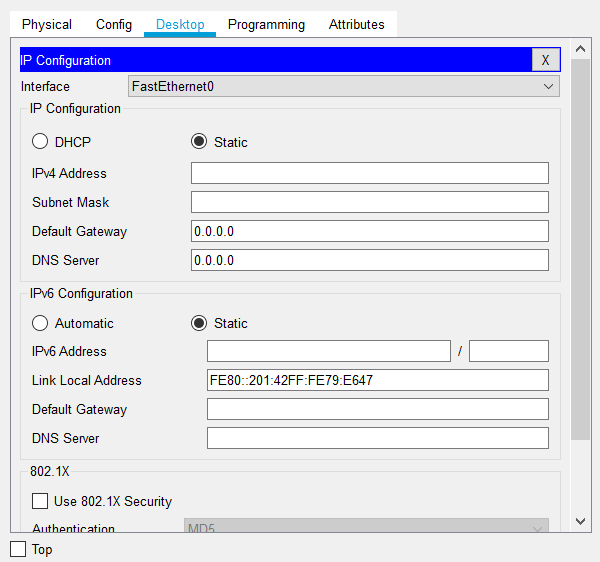
\includegraphics[frame, scale=1]{./Figures/pcsetting.png}
        \caption{IP configuration application present in the desktop of individual PCs}
        \label{fig:pcsetting}
    \end{figure}
    \addtocontents{lol}{\protect\subsubsection*{Sub activity 2}}
    \addtocontents{lot}{\protect\subsubsection*{Sub activity 2}}
    \subsubsection*{Sub activity 2}
    \cmdop{a_a01}{ping test from PC0 to PC1}
    \cmdop{a_a03}{ping test from PC0 to PC3}
    \begin{table}[H]
      \centering
      \ping{
        \multirow{5}{*}{PC0} & PC1 & \multirow{5}{*}{Successful}\\
        & PC2 &\\
        & PC3 &\\
        & PC4 &\\
        & PC5 &\\
      }
  \caption{Observation for ping tests from PC0 to other PCs}
  \label{tbl:activitya0}
  \end{table}
    \addtocontents{lol}{\protect\subsubsection*{Sub activity 3}}
    \addtocontents{lot}{\protect\subsubsection*{Sub activity 3}}
    \subsubsection*{Sub activity 3}
    \cmdop{a_a30}{ping test from PC3 to PC0}
    \cmdop{a_a34}{ping test from PC3 to PC4}
    \begin{table}[H]
      \centering
      \ping{
        \multirow{5}{*}{PC3} & PC0 & \multirow{5}{*}{Successful} \\
        & PC1 &\\
        & PC2 & \\
        & PC4 & \\
        & PC5 & \\
      }
  \caption{Observation for ping tests from PC3 to other PCs}
  \label{tbl:activitya1}
  \end{table}
    \addtocontents{lol}{\protect\subsubsection*{Sub activity 4}}
    \addtocontents{lot}{\protect\subsubsection*{Sub activity 4}}
    \subsubsection*{Sub activity 4}
    \cmdop{a_b01}{ping test from PC0 to PC1}
    \cmdop{a_b03}{ping test from PC0 to PC3}
    \begin{table}[H]
      \centering
      \ping{
        \multirow{5}{*}{PC0} & PC1 & \multirow{2}{*}{Successful} \\
        & PC2 & \\
        \cline{2-3}
        & PC3 & \multirow{3}{*}{Request timed out}\\
        & PC4 & \\
        & PC5 & \\
      }
  \caption{Observation for ping tests from PC0 to other PCs}
  \label{tbl:activitya2}
  \end{table}
    The ping requests from PC0 to PC3 and PC0 to PC1 are successful  for sub activity 2, but when the subnet mask of the PCs are changed from 255.255.255.0 to 255.255.255.224, the ping request from PC0 (200.200.20.2) to PC3 (200.200.20.34) fails with a request timed out error, whereas the ping to PC1 remains unchanged. This is beacuse the sending host, in this case, PC0 can't find the destination PC3 in it's subnet. The change in subnet mask causes the two PCs under consideration to be located in different subnets, hence the ping is unsuccessful.
    \addtocontents{lol}{\protect\subsubsection*{Sub activity 5}}
    \addtocontents{lot}{\protect\subsubsection*{Sub activity 5}}
    \subsubsection*{Sub activity 5}
    \cmdop{a_b30}{ping test from PC3 to PC0}
    \cmdop{a_b34}{ping test from PC3 to PC4}
    \begin{table}[H]
      \centering
      \ping{
        \multirow{5}{*}{PC3} & PC0 & \multirow{3}{*}{Request timed out} \\
        & PC1 & \\
        & PC2 & \\
        \cline{2-3}
        & PC4 & \multirow{2}{*}{Successful}\\
        & PC5 & \\
      }
  \caption{Observation for ping tests from PC3 to other PCs}
  \label{tbl:activitya3}
  \end{table}
  The ping requests from PC3 to PC0 and PC3 to PC4 are successful  for sub activity 3, but when the subnet mask of the PCs are changed from 255.255.255.0 to 255.255.255.224, the ping request from PC3 (200.200.20.34) to PC0 (200.200.20.2) fails with a request timed out error, whereas the ping to PC4 remains unchanged. This is beacuse the sending host, in this case, PC3 can't find the destination PC0 in it's subnet. The change in subnet mask causes the two PCs under consideration to be located in different subnets, hence the ping is unsuccessful.
    \addtocontents{lol}{\protect\subsection*{Activity B}}
    \addtocontents{lot}{\protect\subsection*{Activity B}}
    \subproblem{Activity B}
    The network shown in Figure~\ref{fig:activityb} is extended from the network for Activity A. The router is connected between the two switches using the gigbitethernet ports on the router and fast ethernet ports on the switches.
    \subsubsection*{Sub activity 1}
    \addtocontents{lol}{\protect\subsubsection*{Sub activity 1}}
    \addtocontents{lot}{\protect\subsubsection*{Sub activity 1}}
    The gigabitethernet ports are configured as,
    \begin{table}[H]
        \centering
        \begin{threeparttable}
        \setting{Gigabitethernet}{
        0/0 & 200.200.20.1  & 255.255.255.224 \\
        0/1 & 200.200.20.33  & 255.255.255.224 \\
       }
  \begin{tablenotes}
    \small
    \item Note: The ip addressess and subnet masks are set using the configuration commands shown in Listing~\ref{lst:gigasetb}
  \end{tablenotes}
  \caption{IP address and subnet masks for the gigabitethernet interfaces on Router0}
  \label{tbl:gigasettingb}
        \end{threeparttable}
    \end{table}
    \begin{mdframed}[backgroundcolor=bg,innerbottommargin=-2.5em]
        \lstinputlisting[label={lst:gigasetb},captionpos=b,style=DOS,caption={Syntax for configuring interfaces on Router0}]{./Outputs/gigasetb.txt}
          \end{mdframed}

    \addtocontents{lol}{\protect\subsubsection*{Sub activity 2}}
    \addtocontents{lot}{\protect\subsubsection*{Sub activity 2}}
    \subsubsection*{Sub activity 2}
    \cmdop{b_a01}{ping test from PC0 to PC1}
    \cmdop{b_a03}{ping test from PC0 to PC3}
    \begin{table}[H]
      \centering
      \ping{
        \multirow{5}{*}{PC0} & PC1 & \multirow{2}{*}{Successful} \\
        & PC2 & \\
        \cline{2-3}
        & PC3 & \multirow{3}{*}{Request timed out}\\
        & PC4 & \\
        & PC5 & \\
      }
  \caption{Observation for ping tests from PC0 to other PCs}
  \label{tbl:activityb0}
  \end{table}

    \addtocontents{lol}{\protect\subsubsection*{Sub activity 3}}
    \addtocontents{lot}{\protect\subsubsection*{Sub activity 3}}
    \subsubsection*{Sub activity 3}
    \cmdop{b_a30}{ping test from PC3 to PC0}
    \cmdop{b_a34}{ping test from PC3 to PC4}
    \begin{table}[H]
      \centering
      \ping{
        \multirow{5}{*}{PC3} & PC0 & \multirow{3}{*}{Request timed out} \\
        & PC1 & \\
        & PC2 & \\
        \cline{2-3}
        & PC4 & \multirow{2}{*}{Successful}\\
        & PC5 & \\
      }
  \caption{Observation for ping tests from PC3 to other PCs}
  \label{tbl:activityb1}
    \end{table}

    \addtocontents{lol}{\protect\subsubsection*{Sub activity 4}}
    \addtocontents{lot}{\protect\subsubsection*{Sub activity 4}}
    \subsubsection*{Sub activity 4}
    \cmdop{b_b01}{ping test from PC0 to PC1}
    \cmdop{b_b03}{ping test from PC0 to PC3}
    \begin{table}[H]
      \centering
      \ping{
        \multirow{5}{*}{PC0} & PC1 & \multirow{5}{*}{Successful}\\
        & PC2 &\\
        & PC3 &\\
        & PC4 &\\
        & PC5 &\\
      }
  \caption{Observation for ping tests from PC0 to other PCs}
  \label{tbl:activityb2}
  \end{table}
  The ping request from PC0 to PC1 is successful and PC0 to PC3 failed with request timed out error for sub activity 2, but when the default gateway for PC0, PC1 and PC2 is set to 200.200.20.1 and that for PC3, PC4 and PC5 is set to 200.200.20.33, the ping request from PC0 (200.200.20.2) to PC3 (200.200.20.34) succeeds whereas the ping to PC1 remains unchanged. This is beacuse the sending host, at first couldn't locate PC3 in it's subnet but didn't know where to forward the packet. But once the default gateway is set correctly such that the router can receive the packet in case the sending host doesn't locate the destination itself, the router routes the packets correctly to other subnet. The default gateways for the two subnets are the IP addresses of the interfaces of the router that the switches are connected to. \pagebreak

    \addtocontents{lol}{\protect\subsubsection*{Sub activity 5}}
    \addtocontents{lot}{\protect\subsubsection*{Sub activity 5}}
    \subsubsection*{Sub activity 5}
    \cmdop{b_b30}{ping test from PC3 to PC0}
    \cmdop{b_b34}{ping test from PC3 to PC4}
    \begin{table}[H]
      \centering
      \ping{
        \multirow{5}{*}{PC3} & PC0 & \multirow{5}{*}{Successful} \\
        & PC1 &\\
        & PC2 & \\
        & PC4 & \\
        & PC5 & \\
      }
  \caption{Observation for ping tests from PC3 to other PCs}
  \label{tbl:activityb3}
  \end{table}
  The ping request from PC3 to PC4 is successful and PC3 to PC0 failed with request timed out error for sub activity 3, but when the default gateway for PC0, PC1 and PC2 is set to 200.200.20.1 and that for PC3, PC4 and PC5 is set to 200.200.20.33, the ping request from PC3 (200.200.20.34) to PC0 (200.200.20.2) succeeds whereas the ping to PC4 remains unchanged. This is beacuse the sending host, at first couldn't locate PC0 in it's subnet but didn't know where to forward the packet. But once the default gateway is set correctly such that the router can receive the packet in case the sending host doesn't locate the destination itself, the router routes the packets correctly to other subnet. 

    \addtocontents{lol}{\protect\subsubsection*{Sub activity 6}}
    \subsubsection*{Sub activity 6}
    \cmdop{b_showip}{show ip route on Router0}
    Listing~\ref{lst:b_showip} shows the results for running the show ip route command on Router0. There are two interfaces connected in the network that are denoted by L (Local). Also, C (Connected) status indicates that the route was learned as a result of configuring the interface, which means that the two subnets connected on the two gigabitethernet interfaces are shown. There is no static route available as we haven't set one yet.
    \subproblem{Activity C}
    \addtocontents{lol}{\protect\subsection*{Activity C}}
    \addtocontents{lot}{\protect\subsection*{Activity C}}
    \subsubsection*{Sub activity 1}
    \addtocontents{lot}{\protect\subsubsection*{Sub activity 1}}
    The IP addressess and subnet masks for each PC added are configured as,
    \begin{table}[H]
        \centering
        \begin{threeparttable}
        \setting{PC}{
        6 & 200.200.20.100  & 255.255.255.224 \\
        7 & 200.200.20.101  & 255.255.255.224 \\
        8 & 200.200.20.102  & 255.255.255.224 \\
       }
  \begin{tablenotes}
    \small
    \item Note: The ip addressess and subnet masks are set using the IP configuration application as shown in Figure~\ref{fig:pcsetting}. The default gateway for these PCs is set to 200.200.20.99
  \end{tablenotes}
  \caption{IP address and subnet masks for the PCs added in the network}
  \label{tbl:pcsettingc}
        \end{threeparttable}
    \end{table}
    \subsubsection*{Sub activity 2}
    \addtocontents{lol}{\protect\subsubsection*{Sub activity 2}}
    \addtocontents{lot}{\protect\subsubsection*{Sub activity 2}}
    The IP addressess and subnet masks for the gigabitethernet interfaces on the routers are configured as,
    \begin{table}[H]
        \centering
        \begin{threeparttable}
        \setting{Gigabitethernet interface}{
        Router0 0/0 & 200.200.20.65  & 255.255.255.224 \\
        Router1 0/0 & 200.200.20.66  & 255.255.255.224 \\
        Router1 0/1 & 200.200.20.99  & 255.255.255.224 \\
       }
  \begin{tablenotes}
    \small
    \item Note: The ip addressess and subnet masks are set using the configuration commands shown in Listing~\ref{lst:gigasetc0} and \ref{lst:gigasetc1}
  \end{tablenotes}
  \caption{IP address and subnet masks for the gigabitethernet interfaces on Router0 and Router1}
  \label{tbl:routersettingc}
        \end{threeparttable}
    \end{table}
    \begin{mdframed}[backgroundcolor=bg,innerbottommargin=-2.5em]
        \lstinputlisting[label={lst:gigasetc0},captionpos=b,style=DOS,caption={Syntax for configuring interfaces on Router0}]{./Outputs/gigasetc0.txt}
          \end{mdframed}
          \begin{mdframed}[backgroundcolor=bg,innerbottommargin=-2.5em]
              \lstinputlisting[label={lst:gigasetc1},captionpos=b,style=DOS,caption={Syntax for configuring interfaces on Router1}]{./Outputs/gigasetc1.txt}
                \end{mdframed}
                \subsubsection*{Sub activity 3}
    \addtocontents{lol}{\protect\subsubsection*{Sub activity 3}}
    \addtocontents{lot}{\protect\subsubsection*{Sub activity 3}}
    The different parameters to be configured on Router0 and Router1 are,
    \begin{table}[H]
        \centering
        \begin{threeparttable}
        \parameter{
        0 & Ashlesh & \multirow{2}{*}{ashlesh} & \multirow{ 2}{*}{407} & \multirow{2}{*}{pandey}\\
        1 & Pandey & & & \\
       }
  \begin{tablenotes}
    \small
    \item Note: The ip parameters are set using the configuration commands shown in Listing~\ref{lst:configure0} and \ref{lst:configure1}
  \end{tablenotes}
  \caption{Configuration parameters for Router0 and Router1}
  \label{tbl:parameter}
        \end{threeparttable}
    \end{table}
    \begin{mdframed}[backgroundcolor=bg,innerbottommargin=-2.5em]
        \lstinputlisting[label={lst:configure0},captionpos=b,style=DOS,caption={Syntax for configuring mentioned parameters on Router0}]{./Outputs/c_configure0.txt}
          \end{mdframed}
          \begin{mdframed}[backgroundcolor=bg,innerbottommargin=-2.5em]
              \lstinputlisting[label={lst:configure1},captionpos=b,style=DOS,caption={Syntax for configuring mentioned parameters on Router1}]{./Outputs/c_configure1.txt}
                \end{mdframed}
                \subsubsection*{Sub activity 4}
    \addtocontents{lol}{\protect\subsubsection*{Sub activity 4}}
    \cmdop{c_showip0}{show ip route on Router0}
    \cmdop{c_showip1}{show ip route on Router1}
    
    \subsubsection*{Sub activity 5}
    \addtocontents{lol}{\protect\subsubsection*{Sub activity 5}}
    \addtocontents{lot}{\protect\subsubsection*{Sub activity 5}}
    \cmdop{c_a1}{ping test from PC0 to PC1}
    \cmdop{c_a3}{ping test from PC0 to PC3}
    \cmdop{c_a6}{ping test from PC0 to PC6}
    \cmdop{c_ar0}{ping test from PC0 to Router0 0/0}
    \cmdop{c_ar1}{ping test from PC0 to Router0 0/1}
    \cmdop{c_ar2}{ping test from PC0 to Router0 0/2}
    \cmdop{c_ar3}{ping test from PC0 to Router1 0/0}
    \cmdop{c_ar4}{ping test from PC0 to Router1 0/1}
    \vspace*{-15pt}
    \begin{table}[H]
      \centering
      \ping{
        \multirow{14}{*}{PC0} & PC0 & \multirow{6}{*}{Successful} \\
        & PC1 &\\
        & PC2 & \\
        & PC3 & \\
        & PC4 & \\
        & PC5 & \\
        \cline{2-3}
        & PC6 & \multirow{3}{*}{Destination host unreachable}\\
        & PC7 & \\
        & PC8 & \\
        \cline{2-3}
        & Router0 0/0 & \multirow{3}{*}{Successful}\\
        & Router0 0/1 & \\
        & Router0 0/2 & \\
        \cline{2-3}
        & Router1 0/0 & Request timed out\\
        \cline{2-3}
        & Router1 0/1 & Destination host unreachable\\
      }
  \caption{Observation for ping tests from PC0 to other PCs and router interfaces}
  \label{tbl:activityc5}
  \end{table}
  \vspace*{-12pt}
    \subsubsection*{Sub activity 6}
    \addtocontents{lol}{\protect\subsubsection*{Sub activity 6}}
    \addtocontents{lot}{\protect\subsubsection*{Sub activity 6}}
    \cmdop{c_b0}{ping test from PC3 to PC0}
    \cmdop{c_b4}{ping test from PC3 to PC4}
    \cmdop{c_b6}{ping test from PC3 to PC6}
    \cmdop{c_br0}{ping test from PC3 to Router0 0/0}
    \cmdop{c_br1}{ping test from PC3 to Router0 0/1}
    \cmdop{c_br2}{ping test from PC3 to Router0 0/2}
    \cmdop{c_br3}{ping test from PC3 to Router1 0/0}
    \cmdop{c_br4}{ping test from PC3 to Router1 0/1}

    \begin{table}[H]
      \centering
      \ping{
        \multirow{14}{*}{PC3} & PC0 & \multirow{6}{*}{Successful} \\
        & PC1 &\\
        & PC2 & \\
        & PC3 & \\
        & PC4 & \\
        & PC5 & \\
        \cline{2-3}
        & PC6 & \multirow{3}{*}{Destination host unreachable}\\
        & PC7 & \\
        & PC8 & \\
        \cline{2-3}
        & Router0 0/0 & \multirow{3}{*}{Successful}\\
        & Router0 0/1 & \\
        & Router0 0/2 & \\
        \cline{2-3}
        & Router1 0/0 & Request timed out\\
        \cline{2-3}
        & Router1 0/1 & Destination host unreachable\\
      }
  \caption{Observation for ping tests from PC3 to other PCs and router interfaces}
  \label{tbl:activityc6}
  \end{table}

    \subsubsection*{Sub activity 7}
    \addtocontents{lol}{\protect\subsubsection*{Sub activity 7}}
    \addtocontents{lot}{\protect\subsubsection*{Sub activity 7}}
    \cmdop{c_c0}{ping test from PC6 to PC0}
    \cmdop{c_c3}{ping test from PC6 to PC3}
    \cmdop{c_c7}{ping test from PC6 to PC7}
    \cmdop{c_cr0}{ping test from PC6 to Router0 0/0}
    \cmdop{c_cr1}{ping test from PC6 to Router0 0/1}
    \cmdop{c_cr2}{ping test from PC6 to Router0 0/2}
    \cmdop{c_cr3}{ping test from PC6 to Router1 0/0}
    \cmdop{c_cr4}{ping test from PC6 to Router1 0/1}

    \begin{table}[H]
      \centering
      \ping{
        \multirow{14}{*}{PC6} & PC0 & \multirow{6}{*}{Destination host unreachable} \\
        & PC1 &\\
        & PC2 & \\
        & PC3 & \\
        & PC4 & \\
        & PC5 & \\
        \cline{2-3}
        & PC6 & \multirow{3}{*}{Successful}\\
        & PC7 & \\
        & PC8 & \\
        \cline{2-3}
        & Router0 0/0 & \multirow{2}{*}{Destination host unreachable}\\
        & Router0 0/1 & \\
        \cline{2-3}
        & Router0 0/2 & Request timed out\\
        \cline{2-3}
        & Router1 0/0 & \multirow{2}{*}{Successful}\\
        & Router1 0/1 & \\
      }
  \caption{Observation for ping tests from PC6 to other PCs and router interfaces}
  \label{tbl:activityc7}
  \end{table}

    \subsubsection*{Sub activity 8}
    \addtocontents{lol}{\protect\subsubsection*{Sub activity 8}}
    \addtocontents{lot}{\protect\subsubsection*{Sub activity 8}}
    \cmdop{c_d0}{ping test from Router0 to PC0}
    \cmdop{c_d3}{ping test from Router0 to PC3}
    \cmdop{c_d6}{ping test from Router0 to PC6}
    \cmdop{c_dr0}{ping test from Router0 to Router1 0/0}
    \cmdop{c_dr1}{ping test from Router0 to Router1 0/1}
    
    \begin{table}[H]
      \centering
      \ping{
        \multirow{11}{*}{Router0 (Ashlesh)} & PC0 & \multirow{6}{*}{Successful} \\
        & PC1 &\\
        & PC2 & \\
        & PC3 & \\
        & PC4 & \\
        & PC5 & \\
        \cline{2-3}
        & PC6 & \multirow{3}{*}{Failed}\\
        & PC7 & \\
        & PC8 & \\
        \cline{2-3}
        & Router1 0/0 & Successful\\
        \cline{2-3}
        & Router1 0/1 & Failed\\
      }
  \caption{Observation for ping tests from Router0 to PCs and Router1 interfaces}
  \label{tbl:activityc8}
  \end{table}

    \subsubsection*{Sub activity 9}
    \addtocontents{lol}{\protect\subsubsection*{Sub activity 9}}
    \addtocontents{lot}{\protect\subsubsection*{Sub activity 9}}
    \cmdop{c_e0}{ping test from Router1 to PC0}
    \cmdop{c_e3}{ping test from Router1 to PC3}
    \cmdop{c_e6}{ping test from Router1 to PC6}
    \cmdop{c_er0}{ping test from Router1 to Router0 0/0}
    \cmdop{c_er1}{ping test from Router1 to Router0 0/1}
    \cmdop{c_er2}{ping test from Router1 to Router0 0/2}

    \begin{table}[H]
      \centering
      \ping{
        \multirow{12}{*}{Router1 (Pandey)} & PC0 & \multirow{6}{*}{Failed} \\
        & PC1 &\\
        & PC2 & \\
        & PC3 & \\
        & PC4 & \\
        & PC5 & \\
        \cline{2-3}
        & PC6 & \multirow{3}{*}{Successful}\\
        & PC7 & \\
        & PC8 & \\
        \cline{2-3}
        & Router0 0/0 & \multirow{2}{*}{Failed}\\
        & Router0 0/1 & \\
        \cline{2-3}
        & Router0 0/2 & Successful\\
      }
  \caption{Observation for ping tests from Router1 to PCs and Router0 interfaces}
  \label{tbl:activityc9}
  \end{table}

  \subsubsection*{Sub activity 10}
  \addtocontents{lol}{\protect\subsubsection*{Sub activity 10}}
  \addtocontents{lot}{\protect\subsubsection*{Sub activity 10}}
  The syntax to configure a static ip route is enlisted in Listing~\ref{lst:syntaxrouting}. For the network 3, the subnet mask is 255.255.255.224 and the next-hop-address is 200.200.20.66, but the destination network address needs to be calculated. To calculate the network address for network 3, we can perform bitwise AND operation between the subnet mask for the network and an IP address from the network, i.e. IP address of any of PC6, PC7 or PC8. 
  \begin{table}[H]
    \centering
    \begin{tabular}{C{2cm}C{10cm}}
      \toprule
      \multirow{2}{*}{IP address} & 200.200.20.100 \\
      \cline{2-2}
       & 11001000.11001000.00010100.01100100\\
       \midrule
       Subnet mask &  11111111.11111111.11111111.11100000 \\
        \midrule
        \multirow{2}{*}{Network ID}  & 11001000.11001000.00010100.01100000\\
        \cline{2-2}
        & 200.200.20.96 \\
        \bottomrule
     \end{tabular}
\caption{Calculating network identifier for network 3}
\label{tbl:networkidactivityc}
\end{table}

\begin{mdframed}[backgroundcolor=bg,innerbottommargin=-2.5em]
  \lstinputlisting[label={lst:static0},captionpos=b,style=DOS,caption={Syntax for configuring static route for network 3 on Router0}]{./Outputs/c_f0.txt}
    \end{mdframed}

    \subsubsection*{Sub activity 11}
    \addtocontents{lol}{\protect\subsubsection*{Sub activity 11}}
    The syntax to configure a static ip route is enlisted in Listing~\ref{lst:syntaxrouting}. For both network 1 and network 2, the subnet mask is 255.255.255.224 and the next-hop-address is 200.200.20.65, but the destination network addresses are different which have already been calculated in Table~\ref{tbl:subnetting}.

    \begin{mdframed}[backgroundcolor=bg,innerbottommargin=-2.5em]
      \lstinputlisting[label={lst:static1},captionpos=b,style=DOS,caption={Syntax for configuring static route for network 1 and network 2 on Router1}]{./Outputs/c_f1.txt}
        \end{mdframed}

        \subsubsection*{Sub activity 12}
        \addtocontents{lol}{\protect\subsubsection*{Sub activity 12}}
        \addtocontents{lot}{\protect\subsubsection*{Sub activity 12}}

        \cmdop{c_showip2}{show ip route on Router0}
        \cmdop{c_showip3}{show ip route on Router1}

        On re-running \textit{show ip config} on both the routers, changes in the list are observed. There are additional static routes on both the list. These static routes are key observations since they'll be responsible for routing the packets that were not going through in previous runs. 

        \cmdop{c_g6}{ping test from PC0 to PC6}
        \cmdop{c_gr0}{ping test from PC0 to Router1 0/0}
        \cmdop{c_gr1}{ping test from PC0 to Router1 0/1}

        \begin{table}[H]
          \centering
          \ping{
            \multirow{14}{*}{PC0} & PC0 & \multirow{14}{*}{Successful} \\
            & PC1 &\\
            & PC2 & \\
            & PC3 & \\
            & PC4 & \\
            & PC5 & \\
            & PC6 & \\
            & PC7 & \\
            & PC8 & \\
            & Router0 0/0 & \\
            & Router0 0/1 & \\
            & Router0 0/2 & \\
            & Router1 0/0 & \\
            & Router1 0/1 & \\
          }
      \caption{Observation for ping tests from PC0 to other PCs and router interfaces}
      \label{tbl:activityc12a}
      \end{table}

        \cmdop{c_h6}{ping test from PC3 to PC6}
        \cmdop{c_hr0}{ping test from PC3 to Router1 0/0}
        \cmdop{c_hr1}{ping test from PC3 to Router1 0/1}

        \begin{table}[H]
          \centering
          \ping{
            \multirow{14}{*}{PC3} & PC0 & \multirow{14}{*}{Successful} \\
            & PC1 &\\
            & PC2 & \\
            & PC3 & \\
            & PC4 & \\
            & PC5 & \\
            & PC6 & \\
            & PC7 & \\
            & PC8 & \\
            & Router0 0/0 & \\
            & Router0 0/1 & \\
            & Router0 0/2 & \\
            & Router1 0/0 & \\
            & Router1 0/1 & \\
          }
      \caption{Observation for ping tests from PC3 to other PCs and router interfaces}
      \label{tbl:activityc12b}
      \end{table}

        \cmdop{c_i0}{ping test from PC6 to PC0}
        \cmdop{c_i3}{ping test from PC6 to PC3}
        \cmdop{c_ir0}{ping test from PC6 to Router0 0/0}
        \cmdop{c_ir1}{ping test from PC6 to Router0 0/1}
        \cmdop{c_ir2}{ping test from PC6 to Router0 0/2}
        
        \vspace*{-20pt}
        \begin{table}[H]
          \centering
          \ping{
            \multirow{14}{*}{PC6} & PC0 & \multirow{14}{*}{Successful} \\
            & PC1 &\\
            & PC2 & \\
            & PC3 & \\
            & PC4 & \\
            & PC5 & \\
            & PC6 & \\
            & PC7 & \\
            & PC8 & \\
            & Router0 0/0 & \\
            & Router0 0/1 & \\
            & Router0 0/2 & \\
            & Router1 0/0 & \\
            & Router1 0/1 & \\
          }
      \caption{Observation for ping tests from PC6 to other PCs and router interfaces}
      \label{tbl:activityc12c}
      \end{table}

        \cmdop{c_j6}{ping test from Router0 to PC6}
        \cmdop{c_jr0}{ping test from Router0 to Router1 0/1}

        \begin{table}[H]
          \centering
          \ping{
            \multirow{11}{*}{Router0 (Ashlesh)} & PC0 & \multirow{11}{*}{Successful} \\
            & PC1 &\\
            & PC2 & \\
            & PC3 & \\
            & PC4 & \\
            & PC5 & \\
            & PC6 & \\
            & PC7 & \\
            & PC8 & \\
            & Router1 0/0 & \\
            & Router1 0/1 & \\
          }
      \caption{Observation for ping tests from Router0 to PCs and Router1 interfaces}
      \label{tbl:activityc12d}
      \end{table}

        \cmdop{c_k0}{ping test from Router1 to PC0}
        \cmdop{c_k3}{ping test from Router1 to PC3}
        \cmdop{c_kr0}{ping test from Router1 to Router0 0/0}
        \cmdop{c_kr1}{ping test from Router1 to Router0 0/1}

        \begin{table}[H]
          \centering
          \ping{
            \multirow{12}{*}{Router1 (Pandey)} & PC0 & \multirow{12}{*}{Successful} \\
            & PC1 &\\
            & PC2 & \\
            & PC3 & \\
            & PC4 & \\
            & PC5 & \\
            & PC6 & \\
            & PC7 & \\
            & PC8 & \\
            & Router0 0/0 & \\
            & Router0 0/1 & \\
            & Router0 0/2 & \\
          }
      \caption{Observation for ping tests from Router1 to PCs and Router0 interfaces}
      \label{tbl:activityc12e}
      \end{table}

      The ping tests that previously failed are now successful since the static route has been setup for inter-network communication. The network 1 and 2 can communicate with the default gateway properly set whereas the network 3 requires a proper static route to be accessible from network 1 and network 2 and vice versa. 
      \section{Conclusion}
       The activities were performed sequentially which aided in the understanding of a network subnetting and the various steps that need to be followed to configure a proper network topology. While performing activity A, the concepts of subnet masks and subnetting were understood once the change in the default subnet mask was made. The change divided the network into two subnets which resulted in the ping tests from one subnet to the other to fail. During activity B, the inital observations were quite similar to that of the latter half of activity A since the packets weren't leaving a subnet although we had a router configured. Once the proper default gateways (IP address of the interface connected to the subnet) for all the PCs in both the subnets were set, the two subnets could communicate with each other as seen in the observations. For activity C, two routers were connected and different ping tests were performed. The additional subnetwork 3 couldn't communicate with the existing networks 1 and 2. The ip route table for both the routers showed that the router had no idea of the route that it should forward the packets to, and this is true since the static route wasn't set till this point. This is where the two ways a data packet is sent from a sending host to a destination was observed. Since the host couldn't find the destination on it's subnet, it forwarded the packet to the default gateway, which should've routed the packets to the destination but couldn't since the route wasn't defined. Once the static routes for both the routers were set properly, all the ping tests succeeded. Hence, the completion of this lab experiment allowed us to observe and understand the concepts of subnet masks, default gateway and static routing along with their usage within a network.
\end{document}